\documentclass[a4paper]{article}

\usepackage[margin=2.5cm,headheight=50pt,includeheadfoot]{geometry}

\usepackage{amsfonts}
\usepackage{amsmath}
\usepackage{graphicx}
\usepackage{fancyhdr}
\pagestyle{fancy}
\renewcommand{\headrulewidth}{2pt}

\usepackage{xcolor}

\rhead{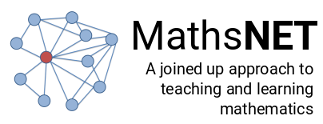
\includegraphics[width=5cm]{../../html/assets/img/logo.png}}
\lhead{\Huge SOR3012: Tutorial week 10}

\begin{document}

\section{Aim}

The aim of the tutorial this week is to try to understand Markov chains in continuous time and the differential equations that have to be solved in order to understand this class of problems.

\section{Bring}

Please bring your notes for the module and suitable items of stationery.

\section{Approach}

It is extremely important to understand how the poisson process is derived as many more complicated continuous time Markov chain are derived by making modifications to this derivation and by relaxing 
the various assumptions that are made in the derivation of the Poisson process.  In this tutorial you will thus spend 20 minutes trying to work through the derivation yourself.  I will then allow you 
to discuss what you tried in small groups and will go around to discuss the problem with those groups that are struggling.  You can (and should) use all your notes on this module as you try to work 
through the problems.

The Poisson process is a continuous time Markov chain that can be used to model the number of events that happen during a fixed interval in time.  In deriving this model we make the following three 
assumptions about the number of events, $N(t)$, that happen in a time interval of length $t$:
$$
\begin{aligned}
 N(0) & = 0 \\
 \lim_{t \rightarrow 0} P\{ N(t)=1 \} & = \lambda \\
 \lim_{t \rightarrow 0} P\{ N(t)>1 \} & = 0 \\
\end{aligned}
$$
Here $P$ is used to indicate a probability measure.  Discuss the following questions:

\begin{enumerate}
 \item Draw a transition graph for the Poisson process and write out the jump rate matrix for this continuous time Markov chain.
 \item Use the Kolmogorov relation and the jump rate matrix you derived in part (1) to show that 
 $$
  \frac{\textrm{d}P_{00}}{\textrm{d}t} = -\lambda P_{00}(t) \qquad \textrm{and} \qquad \frac{\textrm{d}P_{0n}}{\textrm{d}t} = \lambda p_{0(n-1)}(t) - \lambda p_{0n}(t)
 $$
 \item Solve the two differential equations you derived in part (2) and hence show that:
  $$
   p_{0n}(t) = \frac{(\lambda t)^n}{n!} e^{-\lambda t}
  $$
 \item Discuss the approximations that are made about the time between the events that are made in this derivation.  How might you relax this approximation.  Hint: look at the theory of semi-Markov 
chains.

 \item Discuss an example of a problem when it is appropriate to use an inhomogeneous poisson process rather than a homogeneous Poisson process.
\end{enumerate}





\end{document}
